% !TEX program = xelatex
% Minimal validation paper v10 (priority-claim draft), ACM/FSE-style proceedings format.
% Build:  $env:TECTONIC_CACHE_DIR='...\tools\tectonic\cache'; .\tools\tectonic\tectonic.exe -r 3 paper-fse-v10.tex
% Convention: red [TODO: ...] marks are unfilled slots.
% Lineage: v4 is the version reviewed by paper-fse-v4-preprint-review-20261026.md (sha 475e0933...),
% kept byte-identical to that snapshot. v5 = v4 + review items R01-R11. v6 = v5 + items V01-V05 of
% paper-fse-v5-review (the same defects re-examined at the sentence-to-artifact level). v7 = v6 +
% editorial items B (delete) and C (move) of paper-fse-v6-review; no claim changes, no number changes.
% v8 = v7 (as rebuilt by paper-fse-v7-preprint-review-20261026, which fixed the 163k/60KB/six-words
% numbers) + the two provenance defects of that review that can mislead a reader who recomputes.
%
% v7 -> v8 changes:
%   R02  S6.2: the accuracy crossing 6.76 -> 4.20 was attributed to "this intervention", i.e. to the
%        3,584 -> 5,120 update P1 intervention of the paragraph above. It is not that pair: 6.76 is the
%        2,304-update canonical-probe adapter (rd_2304 / m31_rd_2304.pt, the one that scored 0.969) and
%        4.20 is the 5,120-update covered adapter (rd_covered / m38_rdcovered.pt, the one that scored
%        0.84375). Recomputed from per-question scores: 6.7573 and 4.1961 (.local-8b/rstar_from_scores.py).
%        The sentence now names both adapters and says explicitly that this is a different pair from the
%        P1 intervention. 4.19 -> 4.20 for correct rounding of 4.1961; the factor 1.61 is unchanged.
%   R05b .local-8b/m30_acc.py: the crossing test had the sign of the scan inverted (caps run widest ->
%        narrowest, so SR-RD goes + -> -), and its early exit fired on a > 0, so every arm was recorded as
%        "SR already below RD at the widest cap". Fixed to a > 0 >= b; no GPU rerun; no reported number
%        depends on the broken field. Correction recorded in the script header.
%   R05c S4.7 (Data Availability): "statistics scripts are frozen by SHA" is no longer literally true after
%        R05b, so it now carries "apart from one documented correction to a post-hoc crossing test".
%   R01  S1.4 contribution (1): the demand sentence asserted that the information that must cross a
%        boundary grows with the number of compactions K. Made conditional ("when ... grows with the
%        session"), per the author's correction: the bottleneck identification stands as the core insight,
%        but growth of demand is a hypothesis, not a measurement. The contribution title is unchanged.
%
% v8 -> v9 changes (five sentence-level defects found by the author reading the PDF):
%   S1  S6.1(1): dropped "so this is an absence of a detected effect, not evidence that the teacher is
%       unaffected" - the preceding clause (interval compatible with both directions) already says it.
%   S2  S6.3: dropped "that is a structural argument, not a measurement" - the subsection is titled
%       "An Implication We Have Not Tested", so the label was a third statement of the same thing.
%   S3  S6.4(7): the amortisation sentence now cites Doc-to-LoRA, whose contribution is the hypernetwork
%       that amortises the write.
%   S4  S7.1: dropped "which is a comparison of two carriers rather than of a mechanism against its
%       absence". It is false about this paper: Table 4 and Table 5 headline RD against R0, i.e. a carrier
%       against the no-memory baseline. What differs from the compilation family is the trigger and the
%       swept text budget, and the sentence still says that.
%   S5  S7.1/S7.2: the 46.4% conflict cost of Doc-to-LoRA-style methods was in the TMEM subsection; moved
%       to the end of S7.1, the subsection about that family. S7.2 now ends on its own point (the
%       supervision channel).
%
% v9 -> v10 changes (four arithmetic/provenance defects that survive recomputation from the run ledger
% 实验结论.md and r-star及后续实验阶段报告-2026-10-26.md; everything else in the audit lists was
% adjudicated as taste, ledger-supported, or false positive - see V10-CHANGES.md):
%   A2  S1.1: "three orders larger" -> "more than two orders larger". 125 MB / 375 KB = 333x = 2.52 orders;
%       the sentence sits in the paragraph that says "the order of magnitude is the point".
%   A6  附录A "Write budget": 0.32 is the trained-wordings column, 0.220 (next sentence) is the 40-question
%       column. Labelled. Source table: r-star report L143-148, whose own note warns that the two
%       evaluations have different denominators.
%   A7  S1.4, S3.3: dropped "smallest" from "smallest and most auditable": the paper itself scanned rank 16
%       (1,441,792 params) against the 5,767,168 shipped. 实验结论.md L9 records that scan.
%   A8  附录A "Crossing": "The same bracket logic" named an operation S5.2 refuses ("we do not interpolate a
%       single value"). Now says log-r interpolation, and states the sampled bracket (512/1024-token
%       budgets = two to eight times ours) next to the interpolated 540-650. Table 9's cell now says
%       "interpolated", and S6.2's "two to five times our own" is now "two to eight" so the two places
%       quote the same quantity.
%   A10 附录A "Coverage": 173 s / 224 s were labelled "Cost of the second"; the only sources call them the
%       incremental cost of the 24 added probes. Relabelled.
%
% v6 -> v7 changes (all deletions/moves; every headline claim survives its own sentence):
%   B1  Intro: "We do not test this bias hypothesis here." (previous sentence already scopes it).
%   B2  S3.5: ", and we do not claim they are" (the preceding clause states the units differ).
%   B3  S5.1 Takeaway: ", and we do not report a single number for it" (interval crossing zero said).
%   B4  S5.2: "this is not a result in which our method wins; it localizes where it stops losing".
%   B5  S5.3: "and no such bound is claimed" (after "does not identify an intrinsic lower bound").
%   B6  S6.1(2): "(per-cell values in the artifact, not reproduced here)" - an unverifiable pointer.
%       OPEN: the per-cell values are not in .local-8b under any template/heading key; see V07 note
%       in V7-CHANGES.md before claiming this passage is backed by a table.
%   B7  S6.2: "and we do not read rank as ruled out" (third synonym after two other negations).
%   B8  S6.3: dropped the second and third restatements of the same negation; the paragraph now ends
%       at "a structural argument, not a measurement".
%   B9  S7.4: ", and we do not claim it does".
%   B10 S7.4: "We do not repeat ``parameters are stronger'';".
%   B11 S5.2: dropped "we treat the sweep as conditional on one summary construction policy / did not
%       run truncation instead of regeneration"; the two confounds that remain are the r=19.8 reuse
%       and the cap-64 truncation. NOTE: this removes the only place the paper says regeneration vs
%       truncation was not separated; see V7-CHANGES.md before freezing.
%   C1  Moved S5.3 "What we did not measure" into S8 as "Measured, and not measured", placed between
%       External and Scope of the runs. S5.3 now runs: cost -> rehearsal -> what the rows separate ->
%       Takeaway. RQ3 now points there; S6.4 item 4's duplicate sentence was dropped.
%   C2  S6.4 item 3 (probe set) compressed from nine sentences to two, pointing at S8 (new label
%       sec:threats), where Internal (i) carries the long form.

\documentclass[sigconf,nonacm]{acmart}

\usepackage{amsmath}
\providecommand{\checkmark}{\ensuremath{\surd}}
\usepackage{array}
\usepackage{tabularx}
\usepackage{booktabs}
\usepackage{xcolor}
\usepackage{enumitem}

% Inline formulas leave few breakpoints in some paragraphs; allow extra stretch
% rather than letting text run past the column edge.
\setlength{\emergencystretch}{1.5em}

\settopmatter{printacmref=false}
\setcopyright{none}
\renewcommand\footnotetextcopyrightpermission[1]{}
\pagestyle{plain}

\newcommand{\todo}[1]{\textcolor{red}{\textbf{[TODO: #1]}}}
\newcommand{\KL}{\mathrm{KL}}
\newcommand{\St}{\texttt{SR}}
\newcommand{\Sd}{\texttt{SRD}}
\newcommand{\armT}{\texttt{T}}
\newcommand{\armR}{\texttt{R0}}
\newcommand{\armRD}{\texttt{RD}}

\begin{document}

\title{Remember Rather Than Hand Off:\\
Mid-Speed Weights for Cross-Compaction Continuity}

% Double-blind review build: switch the class line above to
%   \documentclass[sigconf,nonacm,anonymous]{acmart}
% which makes acmart suppress all author information. The default build below is the
% named (arXiv / camera-ready) version.
\author{Mingjie Zeng}
\affiliation{%
  \institution{State Key Laboratory for Novel Software Technology, Nanjing University}
  \country{China}}
\email{357400942@qq.com}

\author{Xin Zhou}
\authornote{Corresponding author.}
\affiliation{%
  \institution{State Key Laboratory for Novel Software Technology, Nanjing University}
  \country{China}}
\email{zhouxin@nju.edu.cn}

\author{He Zhang}
\affiliation{%
  \institution{State Key Laboratory for Novel Software Technology, Nanjing University}
  \country{China}}
\email{hezhang@nju.edu.cn}

\begin{abstract}
In long-horizon sessions, history repeatedly crosses a compaction boundary, and what survives is text only: a
summary, a sliding window, or a ledger. Each is billed on every use: with cached dense attention, a carried
$k$-token prefix adds $O(k)$ attention work per decoded position, $O(km)$ over $m$ decoded positions, while a fixed
adapter adds a constant per position and occupies no context positions. Each is also capped---a summary of at most 32k tokens, a sliding window of fixed width---so whatever
survives a compaction is a constant, independent of how much history preceded it, and its capacity, not only
its recurring price, is a ceiling. We
ask whether that carrier can instead be parameters: at the compaction boundary we write the full-context
teacher's output distribution into a session-local, unmerged low-rank $\Delta$ that is bitwise identity when
cleared, and compare it against the output of a \emph{real} compaction engine whose summary budget we sweep
over a $16\times$ range while $\Delta$'s cost is held fixed. On a single
27B model over four histories, $\Delta$ reduces the divergence from the teacher by 25.1/28.0/28.5\% over
the tail-only baseline (a fourth history gives 7.7\%, with an interval crossing zero), and by 17.8\% on top
of a summary in one history; on a 20k-token history the text carrier is better until the summary is compressed
to 128--256 tokens---a 77.5--154.9$\times$ compression of the history---where the comparison reverses; and on
unrelated questions $\Delta$ costs 0.026
nats/position, versus 0.017 for adding a summary. Everything measured here concerns \emph{where} the state
lives, not what it can recall. We report an auditable controlled measurement rather than a
better method.
\end{abstract}

\keywords{conversation memory, context compaction, context distillation, KV cache, parametric
memory, LLM agents}

\maketitle

\section{Introduction: What Is Missing Is a Carrier, Not a Time Scale}

\subsection*{Prologue: they hand off, they do not remember}

An agent works through a long session, the window fills, and the history is compacted: a few hundred
tokens survive, the rest is discarded. What crosses the boundary is not what the agent learned but a
summary of what it said---a handoff to a stranger, repeated at every boundary.

Humans do not do this: sleep consolidates experience into the same substrate that will use it later. Between
an LLM's fast weights---the KV cache \cite{mita2026,schlag2021}---and its frozen weights there is no such
substrate. Following that principle we introduce \textbf{mid-speed weights}, and we call the approach
\textbf{AVCP} (AdVance ComPact). This paper asks whether that middle layer can be written at the compaction
boundary, and what it costs.

\subsection{A Concrete Discontinuity}
Session history in agent systems keeps growing. To keep the context window sustainable, a system
eventually \emph{compacts}: earlier history is compressed into a summary and the raw text is discarded.
The operation is lossy, and for a summary the loss is unverifiable---nobody knows what was dropped. A
ledger that keeps pointers into the original history makes it checkable, at the price of paying per use
(\S\ref{sec:related}); that is a different carrier with a different cost profile, not a fix to the summary.

What is dropped is usually not a task fact. The compaction instruction in our production engine reads
\emph{``Preserve exact file paths, commands, error strings, identifiers, numeric values, function
signatures''}. It names factual categories explicitly, and asks for no preservation of register, sentence
length, or order of judgment. A concrete example: if the user asked early in the session to drop formal
address, and the model complied by token 200k, then what should survive compaction is not the
\emph{rule} ``the user prefers informal address''---which is easy to write into a summary---but the
\textbf{register continuity} created by three hundred informal turns. It is not a task fact but a
disposition threaded through the whole conversation, and it conditions every subsequent answer.

This is an argument about \emph{existing compaction engines}, not a result of this paper: text is
perfectly capable of carrying such information (``the user dislikes honorifics'' is four words); the
current instruction simply does not ask for it. That it is not
a rhetorical worry is supported by analyses of generative compaction, whose minimum budget is
communication-complexity-equivalent \cite{compacttheory2026}, and by measurements in which side
constraints are retained at only 17\% without a bypass ledger \cite{lostincompact2026}.

\paragraph{The ceiling is capacity, not only cost.} We instantiate the text carrier with the production
harness we measure (dsh \cite{dsh}); its compaction keeps a summary of at most 32k tokens plus a sliding
window of $0.16W$, in both the scaled-down 40k preset and the 1M preset. Those constants are that engine's
preset; what they instantiate---a capped, per-use-billed text carrier---is not. A text carrier of $k$ tokens can hold at most $O(k)$
bits. At 3 bits/token---an order-of-magnitude anchor from the entropy of printed English and from language-model
compression rates, not a Shannon measure of these transcripts \cite{shannon1951,deletang2024}---a
one-million-token window is roughly 375~KB, and what survives a compaction is roughly 74~KB. Three limits are
distinct and must not be conflated: the model window $W$ (up to one million tokens here), the summary cap (at
most 32k tokens), and the total that survives one compaction---for a one-million-token preset, on the order of
196k tokens, i.e.\ $0.16W$ plus the cap. The runs in this paper use summaries of about 1k tokens, an order of
magnitude below the cap, which is the favourable case for the text carrier. That ceiling does
not move as the history grows: the hundredth
compaction carries no more than the first. A parameter carrier is a constant too, but of a different
order---5.77M parameters, 11~MiB in BF16 and 22~MiB in FP32, against 33~MiB for the three-projection design
budget---and it is written once, then read at a constant cost per processed token.

For scale, a human is estimated to retain on the order of 125~MB of learned information over a lifetime
\cite{landauer1986}, whereas a one-million-token window holds roughly 300--375~KB at 3 bits/token. The two
figures are measured differently and do not form a capacity equation; the order of magnitude is the point. A
lifetime of human experience is more than two orders larger than what an LLM can carry at once, and unlike human
memory the LLM's carrying capacity does not accumulate: the hundredth compaction carries no more than the
first. That combination---small, and fixed---is the bottleneck this paper is about.

\subsection{``Just Make the Window Bigger'' Runs Out Physically}
In a Qwen3.8-27B-class configuration (64 layers, 16 of which are full attention, 4 KV heads
$\times$ 256 dimensions), the KV cache is
\[
2 \times 16 \times 4 \times 256 \times 2\ \text{B} \;=\; 64\ \mathrm{KiB/token}.
\]
163,840 tokens (about 0.16 of a $2^{20}$ window) of resident KV is 10.0 GiB; 800k tokens is about 49 GiB,
leaving little room on a 96~GB card. (The 48 linear-attention layers carry a separate, length-independent
recurrent state of roughly 144~MiB per sequence in FP32; it is $O(1)$ in $n$ and is not part of the
per-token figure.) Sparsification reduces the constant, not $n$. In other words, enlarging the window is a road that
charges linearly in history length.

\paragraph{KV compression is a real and effective road---it just does not answer our question.}
Long context became practical not because windows grew, but because KV caches were compressed:
DeepSeek-V4.1-Flash reduces the global (HBM-resident) KV cache to \textbf{890 bytes/token}, roughly
$1/4$ of the corresponding V4 footprint, and reduces the persistent part to about $1/8$ via FP4 KV
caching and cross-layer reuse \cite{deepseekv41flash2026}. At that density, one million tokens of
resident KV is about \textbf{0.89 GB}---slightly under 1 GB. LLMs have indeed entered the
million-token era along this path. The Qwen line pushes in the same direction
\cite{qwen3report2025,qwen38report2026}.

This road is a premise of the present work, not its opponent: without it, long sessions would not be
deployable at all. But it addresses a \textbf{constant factor}, not \textbf{whether the information is
there}:

\begin{enumerate}[leftmargin=1.2em]
\item \textbf{Compression is not coverage.} Shrinking the KV cache by $4\times$ does not change whether
the model actually uses the history; if the training distribution contains no pattern of the form
``given this history, answer like this'', a wider window will not produce one.
\item \textbf{The cost is still $O(n)$ up to a constant.} At 890 bytes/token, one million tokens still
occupies 0.89~GB and is scanned for every generated token. A parameter carrier is $O(1)$.
\item \textbf{It is not an oracle.} The KV cache stores the model's activations over a prefix, not the
\emph{correct summary} of that history. It does not say what to keep or drop, and offers no auditable
trade-off.
\end{enumerate}

\paragraph{Degradation at long context is a training-side problem, and not ours.} Long-context degradation
is documented: in a recursive-KV setting, a checkpoint trained at 8k contexts falls to 35.2\% at 128k
\cite{still2026}. Its main causes are the training length distribution and positional generalization, and
this paper does not address them. The boundary of our own probe should be stated explicitly: on 32
unrelated questions we did not detect a degradation of the full-context teacher (\S6.1). That is
consistent rather than contradictory---those questions do not require the far context, and our comparison
is the teacher against $\armR$, not a short-context-trained model against a long one.

We therefore treat KV compression as a solved engineering premise and place our question above it:
\emph{once the window is no longer the bottleneck, in what form should history be carried?}

\subsection{Architecturally There Are Only Two Kinds of Weights}
MiTA \cite{mita2026,schlag2021} observes that standard attention is equivalent to a two-layer fast-weight
MLP whose width is the sequence length, while the FFN is a slow-weight MLP:
\begin{quote}
fast-weight MLP (attention, rewritten at every forward pass) \;+\; slow-weight MLP (FFN, frozen after
pretraining). There is no third kind.
\end{quote}
The dichotomy concerns \emph{weights}: a token carrier is neither fast nor slow; it is an attached
sequence that must still be inflated into fast weights before use. Within this framing there are two forms for
the intermediate band---\textbf{text (status quo) or weights written at the boundary (this paper)}---and the
framing is ours: a fixed-size recurrent state, which some architectures already carry, is a third case we do not
cover (\S\ref{sec:future}).

\subsection{What This Paper Does}
We treat the compaction boundary as a write point and spend one gradient write on a session-local
low-rank $\Delta$. Three contributions:
\begin{enumerate}[leftmargin=1.2em]
\item \textbf{Bottleneck identification.} The intermediate band lacks a carrier, not a time scale. Two
costs accumulate on the text side. \emph{Demand}: when the information that must survive a boundary grows
with the session, a fixed carrier budget becomes a bottleneck---any text carrier is capped at a summary of cap
tokens plus a window of $0.16W$, independent of $K$. \emph{Unit price}: holding the injected length fixed at $k$, a carried
prefix adds $O(k)$ attention work per decoded position and $O(km)$ over $m$ positions, because those $k$ tokens
sit in the attended sequence. A fixed adapter adds a constant per position, occupies no positions, and is written
once. This is a \textbf{cost argument} and is independent of any
particular model.
\item \textbf{An auditable write protocol.} Three invariants---carriers differ, non-carriers are
byte-identical, and $\Delta=0$ is bitwise identity---turn ``parameters versus text'' into a comparison of what each
carrier costs and occupies, at matched tokens, rather than a benchmark race.
\item \textbf{A measurable crossover.} We restate ``can parameters replace text?'' as
\textbf{measuring the compression ratio $r^\ast$} at which the parameter carrier overtakes the text
carrier, instead of arguing about who wins.
\end{enumerate}

\paragraph{What this paper establishes, and what it does not.} The prologue is the thesis, not the result. What
this paper reports is a controlled measurement of it: whether a session-local parameter carrier can be written at
the compaction boundary at all, what it costs, and where it loses to text. It does \emph{not} establish that
mid-speed weights can carry a lifetime of experience, nor that any particular capacity is reachable.

\paragraph{Instantiation versus budget.} The design budget for mid-speed weights is 33~MiB (66~MiB in FP32):
at rank 64 the three FFN projections of the same four layers cost $3\times$ the carrier we ship, 17,301,504
parameters. This version mounts a low-rank additive update on \texttt{down\_proj} of layers 60--63 only:
5,767,168 parameters, 11~MiB in BF16 and 22~MiB in FP32. That is the most auditable carrier; the
larger figure is a design target, not a result.

\section{Background and Preliminaries}

\subsection{The Four Criteria}\label{sec:criteria}

A work addresses the same question as ours only if all hold, with the fourth conditional on the first:
\textbf{(A) Write point}: is the write performed at the moment history is destroyed?
\textbf{(B) Carrier}: does the memory reside in parameters at inference, rather than still appearing in the
context as tokens, soft tokens or KV? That training touched the parameters does not by itself satisfy (B).
\textbf{(C) Supervision}: does the student learn from the teacher's \emph{output distribution}, rather than
from task labels or from targets that were first written out as text? Anything trained on a distribution gets
a tick here, however it is sampled.
\textbf{(A$'$) Lifecycle, defined only when (A) holds}: is the artifact session-local, bitwise-revertible at
$\Delta=0$, and disposable? Where (A) fails the question does not arise, and we write ``n/a''.
Note that (C) is \emph{not} a source of novelty: context distillation has had this form from the start
(\S2.2). (A) and (C) are each individually common: boundary-triggered text compression satisfies (A) without
writing parameters, and document-level compilers satisfy (C) without writing at a boundary. Neither column is
scarce, alone or together with (B). What is scarce is the conjunction.
Covering two or three of the four is the common and reasonable case---each system is designed for the
constraints its own setting poses, and these criteria are not a quality ladder.

\subsection{Relation to Post-Training and Context Distillation}

The obvious objection is: \emph{is this not just distillation post-training with a model that has
already learned something?} \textbf{Yes, the supervision term is exactly that.} The standard form of
context distillation---contextual teacher, context-free student, KL supervision---is structurally
identical to our objective, and Doc-to-LoRA's Eq.~2/4 is literally this \cite{doctolora2026,snell2022}.
We do not claim it as novel. The differences are four:

\begin{enumerate}[leftmargin=1.2em]
\item \textbf{No training happens on the teacher side.} The teacher is not ``a model that learned''; it
is \emph{the same frozen weights with a 20k-token longer prefix}. It is therefore raw material that can
be re-derived per session at zero training cost.
\item \textbf{The default action on the artifact is opposite.} A post-training artifact is expected to be
a \emph{permanent improvement}, and is accepted by asking ``does removing it hurt?''. Our artifact is
expected to be \emph{deleted}, and is accepted by asking ``does removing it restore bitwise identity?''
\item \textbf{The baseline is different.} Post-training is compared against less or no training; we are
compared against \textbf{a real summary over a swept token budget, with a fixed adapter configuration}. The
question is not whether
distillation works, but whether a given budget is better spent on parameters or on tokens.
\item \textbf{The data predict a different follow-up.} If this were post-training, the next step would
be more data and more capacity. We measure that a $4\times$ larger capacity buys only 8 percentage points on
this history. We do \emph{not} conclude that the training budget is irrelevant: within the range we scanned
($\le 16$ passes per probe) the $64\to256$-step increment has an interval crossing zero, but that range is too
narrow to separate the two budgets, and \S\ref{sec:replication} reports a saturated regime in which the budget
dominates.
\end{enumerate}

In one line: \textbf{post-training writes a capability into the model; we are writing its history. The
former must generalize; the latter must be deletable.} There is an informative inversion, too: the
``insufficient generalization'' we measure---directional cross-history transfer, benefits vanishing under
superficial perturbation---is a defect under post-training and \emph{evidence} under a carrier framing.
A $\Delta$ that generalized across histories would be a general-purpose fine-tune, which would be a
failure precisely because it would no longer be bound to this history.

\subsection{Why Supervision Does Not Come from Self-Generated Data}

Our training material is not generated out of thin air: the bulk of $H$ consists of external inputs
(user messages, tool returns, file contents, command output). This is not a stylistic choice.
Multi-round internalization of self-generated experience has been reported as \emph{progressive
capability collapse} rather than compounding \cite{collapse2026}, and the loss of distributional tails
when training on recursively generated data is an earlier and well-known result \cite{shumailov2024}.
Supervision must therefore be anchored on external facts: the teacher's $A$ is external material, and
$\Delta$ fits the distribution it induces.

\subsection{Scale Anchors (Not Interchangeable)}

The following numbers are often placed side by side, but they are measured differently; we use them only
to convey orders of magnitude, and they form no capacity equation: human long-term memory on the order of
$10^{9}$ bits \cite{landauer1986}; printed English entropy 0.6--1.3 bits/character \cite{shannon1951}; a
large model compressing enwik9 to single-digit percentages of its original size \cite{deletang2024}; the
human genome at about $3\times10^{9}$ base pairs \cite{genome}; the human brain at about
$8.61\times10^{10}$ neurons \cite{azevedo2009} and $10^{14}$ synapses \cite{brain}.

\section{Approach: Writing at the Compaction Boundary}

\subsection{Setup and Invariants}\label{sec:notation}

Let $p_\theta$ be the frozen base model, $E$ the system message and tool definitions, and $q$ the current
request. The session history $H$ is split at the compaction boundary into a \emph{block} $A$ (to be
removed) and a \emph{tail} $R$ (retained). The compaction engine is $\mathcal{K}$, whose summary
$S=\mathcal{K}(H)$ satisfies $|S|\le\mathrm{cap}$.

The five arms compared in this paper are defined in \S\ref{sec:arms}; here we fix only the notation.

The bare symbol $R$ always names the retained tail; the no-memory arm always carries its label,
$\armR{}=E{+}R{+}q$. Every $\KL(\cdot\|\cdot)$ below is between model states, never between a state and a
token sequence.

$\Delta$ is a \emph{set} of per-layer additive updates on \texttt{down\_proj} in FFN layers 60--63,
$\Delta\triangleq\{\Delta_l\}_{l\in\{60,\dots,63\}}$ with $\Delta_l=B_lA_l$, rank 64, scale 1, $A_l/B_l$ in
FP32 and $B_l{=}0$ at initialisation; the shipped layer is $W_l' = W_l + \Delta_l$, and $\Delta$ never appears
as a single summed matrix because the factors act on different hidden layers. Thus at $\Delta=0$,
$p_{\theta+\Delta}$ is bitwise identical to $p_\theta$.

Three invariants hold the comparison together; if any is broken, a paired difference cannot be attributed.
\begin{description}[leftmargin=1.2em]
\item[I1 Carriers differ, non-carriers are identical.] $E$, tools, $q$, and any non-carrier instruction are
byte-identical across all arms (including $\armT$); only the pre-registered carrier changes.
\item[I2 Shared carrier components are held fixed.] $S$ is byte-identical across summary arms; boundary, $R$,
$q$ and decode budget are identical. $\Sd-\St$ changes only $\Delta$.
\item[I3 Lifecycle.] The base model is frozen throughout; $\Delta$ is session-local, stored separately, never
merged, and cleared at session end.
\end{description}

\subsection{Writing at the Boundary}

The compaction boundary is chosen for three reasons: (i) it is the only moment at which history is about
to disappear, so what is written corresponds one-to-one with what is lost; (ii) the full-context teacher
$E{+}A{+}R{+}q$ is available, so its distribution can be collected at no extra data cost; (iii) it is a
natural segmentation of the session, which gives the lifecycle of $\Delta$ a well-defined meaning.

That lifecycle follows from the write point rather than being added to it. $\Delta$ is session-local, stored
separately, and never merged into the base model; it is cleared at session end, so there is no cross-session
contamination and no ``residue'' to clean up.

\subsection{Carrier}

The carrier is a per-layer additive low-rank term $\Delta=B_lA_l$ for $l\in\{60,61,62,63\}$ applied to
\texttt{down\_proj}. The form does not affect the principle, only the removal cost and the backward depth:
an unmerged low-rank $\Delta$ of 5,767,168 parameters (11~MiB in BF16, 22~MiB in FP32) can be bypassed and
never touches the base weights, which
makes it the most auditable option.

\subsection{Training Objective}

For each training probe $q_i$ we collect the teacher's full output distribution under $E{+}A{+}R{+}q_i$
and minimize full-vocabulary forward KL over answer positions. Writing $c_i^t = E{+}A{+}R{+}q_i{+}y_{i,<t}$
for the teacher context and $s_i^t = E{+}R{+}q_i{+}y_{i,<t}$ for the student context,
\begin{equation}
\mathcal{L}(\Delta) \;=\; \frac{1}{|\mathcal{Q}|}\sum_{i}\frac{1}{|P_i|}\sum_{t\in P_i}
\KL\!\left( p_\theta(\cdot\mid c_i^t) \,\middle\|\, p_{\theta+\Delta}(\cdot\mid s_i^t) \right)
\label{eq:obj}
\end{equation}
where $P_i$ is the supervision position set and $y_i$ the teacher answer. We run exactly 64 AdamW updates
at learning rate $3\times10^{-4}$ and never select a checkpoint by evaluation result.

We make \textbf{no selection over training positions or training samples}: all answer positions are
supervised and the 16 probes are drawn uniformly. Selective distillation decomposes this dimension into
position/class/sample axes and reports that student-entropy-guided position selection (top-20\%) beats
full-position supervision on both accuracy and perplexity \cite{tavor2026,selectkd2026}; selecting samples
by teacher-student disagreement is a related line \cite{maxdiv2026}. Both presuppose a teacher worth
trusting adaptively, whereas here the teacher is an \emph{empirical reference} rather than an oracle
\cite{adaptivekd2025}. We therefore keep uniform supervision as the baseline and list this axis as
unscanned (\S8). The probe set itself is a placeholder: 16 uniformly drawn probes, with no coverage criterion,
is not a designed sample of a history, and the whole protocol inherits that weakness (\S\ref{sec:limits}).

\subsection{Cost Model}\label{sec:costmodel}

Table~\ref{tab:cost} gives each carrier's cost on the write side and the use side: text carriers pay on the
use side, $\Delta$ pays once on the write side and pays a constant per token thereafter.
\begin{table}[t]
\centering
\small
\begin{tabularx}{\columnwidth}{@{}>{\raggedright\arraybackslash}p{1.5cm}>{\raggedright\arraybackslash}X>{\raggedright\arraybackslash}X@{}}
\toprule
Carrier & Write & Per use \\
\midrule
Full/window $A{+}R$ & none (already paid) & $n$ tokens, $\propto n$ KV \\
Summary $S$ & one full-$H$ call & $\le$cap prefix, occupies window \\
Ledger & one extraction & $k$ injected entries \\
$\Delta$ & one training pass & $O(1)$ extra matmul, no window \\
\bottomrule
\end{tabularx}
\caption{Cost shape of four carriers.}
\label{tab:cost}
\end{table}

Hence the only cost argument in this paper:
\begin{quote}
With cached dense attention and fixed model dimensions, a $k$-token carried prefix adds $O(k)$ attention work per
decoded token and $O(km)$ over $m$ decoded tokens. A fixed unmerged adapter adds a constant amount of computation
per processed token and occupies no context positions. For a fixed adapter configuration its storage and its
per-token computation therefore do not grow with history length, and it adds no text prefix. We do not measure a
common-unit cost comparison, nor equal-fidelity scaling with history length: we vary the text budget at fixed
$|H|$, so a curve of adapter capacity against history length is not measured here.
\end{quote}

No normalization is applied or implied: the two sides are not costed in a common unit. What is held fixed is the supervision input (the same boundary, $R$, $q$ and decode budget); what
is swept is the text carrier's budget. The claim is only that $\Delta$'s cost does not move as that sweep
narrows---not that the two carriers cost the same.

\section{Experimental Design}\label{sec:protocol}

\subsection{Research Questions}

\begin{enumerate}[leftmargin=2.6em,label=\textbf{RQ\arabic*}]
\item \textbf{Fidelity.} Does a session-local $\Delta$ written at the compaction boundary reduce the divergence
between the post-boundary model and the full-context teacher, and by how much on each history? (\S\ref{sec:fit},
Tables~\ref{tab:fit} and~\ref{tab:marginal})
\item \textbf{Location.} At what summary budget does the parameter carrier overtake the text carrier, and is
that location stable across histories? (\S\ref{sec:crossover}, Tables~\ref{tab:threeH} and~\ref{tab:rstar},
Figure~\ref{fig:rstar})
\item \textbf{Price.} What does the write do to questions that do not need the history, can that cost be trained
away, and what is still unmeasured? (\S\ref{sec:cost}, Table~\ref{tab:replay}; the gaps are listed in
\S\ref{sec:threats})
\end{enumerate}

The three questions map one-to-one onto \S5.1--\S5.3, and onto the three contributions of \S1.4.

\begin{table}[t]
\centering
\small
\begin{tabular}{@{}l>{\raggedright\arraybackslash}p{3.9cm}@{}}
\toprule
Knob & Type, and what this paper does \\
\midrule
Compression ratio $r=|H|/|S_{\text{body}}|$ & continuous; five budgets on H20, three on each short history \\
Summary construction & categorical (regenerate at cap vs truncate); not separated \\
$\Delta$ capacity (rank) & integer; 16 and 64 reported, 128 prepared and not run \\
$\Delta$ layer placement & combinatorial, $\binom{64}{k}$; fixed at 60--63, never varied \\
Probe set & \textbf{no parameterisation}; 16 uniform draws, all answer positions \\
Carrier type & binary (low-rank or residual block); low-rank only \\
Write budget & integer; 0/16/64/256 updates, at most 16 passes per probe \\
\bottomrule
\end{tabular}
\caption{The design space: seven knobs, their type, and how far this paper moves each one.}
\label{tab:knobs}
\end{table}

\subsection{Histories and Questions}\label{sec:histories}

All four histories are synthetic agent sessions from one generator, not recorded user sessions. H1--H3 are
three variants of a four-entity, 36-transaction session, each serialized to about 7.1k tokens; the
compaction engine's summary bodies are 1989, 1086 and 1178 tokens respectively, so $r$ differs across them at
an equal cap. H20 is one 19.8k-token session built from 104 structured transactions over 12 entities, with two
summary variants $S_1$ (body 1002 tokens) and $S_2$; the $r$ ladder of \S\ref{sec:results} is swept on this
history, which is also where the unrelated-question cost is measured. Each history supplies 16 training, 8
validation and 64 test questions sharing frozen teacher targets, plus the same 32 unrelated questions. Because
the histories differ in content rather than being replications of one another, a number repeated across them
is not a sample.

The compaction engine never sees the evaluation questions: its summary is produced from the history alone. A
question-aware retrieval policy may change the comparison, and we did not evaluate one, so the crossover we report
is a statement about question-blind compaction, not about retrieval-augmented compaction.

\subsection{Arms and Baselines}\label{sec:arms}

The five arms differ only in the carrier of the history; the tokens they share ($E$, tools, $q$) are
byte-identical across all of them (\S\ref{sec:notation}): $\armT = E{+}A{+}R{+}q$ is the full-context teacher,
$\armR = E{+}R{+}q$ the lower bound with no memory, $\St = E{+}\mathrm{frame}(S){+}R{+}q$ the output of the
compaction engine, $\armRD = E{+}R{+}q{+}\Delta$ the parameterized memory, and
$\Sd = E{+}\mathrm{frame}(S){+}R{+}q{+}\Delta$ the complementary arm.

\paragraph{Compression ratio.} The independent variable of the sweep is $r=|H|/|S_{\text{body}}|$, both terms
measured with the frozen tokenizer. $|S_{\text{body}}|$ excludes the frame and the summary template headers, and
we always report \emph{actual} lengths rather than the cap; for the 20k-token history $r\approx20$, and exact
values are recorded per run.

\subsection{Evaluation Metrics}

Every number below comes from one of three quantities, listed in Table~\ref{tab:metrics}. The first is the
fidelity metric (teacher versus arm); the second measures $\Delta$'s own drift with no teacher in the loop; the
third reads text rather than a distribution. They are never merged, because a small drift is not evidence of
fidelity and a likelihood is not a distribution: the first two compare 248,320-dimensional distributions, the
third compares a single token per position.

\begin{table}[t]
\centering
\small
\begin{tabularx}{\columnwidth}{@{}>{\raggedright\arraybackslash}p{2.3cm}>{\raggedright\arraybackslash}X>{\raggedright\arraybackslash}p{1.7cm}@{}}
\toprule
Quantity & Object vs.\ reference & Use \\
\midrule
$\KL(T\|X)$ & one model state vs.\ another model's full-vocab distribution & fidelity (primary) \\
$\KL(X_{\text{off}}\|X_{\text{on}})$ & one model state vs.\ itself with $\Delta$ off & $\Delta$'s own drift \\
NLL / PPL & one model state vs.\ text as a point mass & summary channel, gold likelihood \\
\bottomrule
\end{tabularx}
\caption{The three metric families.}
\label{tab:metrics}
\end{table}

\paragraph{Position sets and weighting.}

Related questions take answer positions along the \emph{same frozen teacher path}, and all arms share the
same target token ids. The 32 unrelated questions share a fixed gold prefix and contribute 50 scored positions in
total, not 50 each. Scoring averages positions within a question and then weights questions equally; we report
actual position counts, truncation and coverage.

\subsection{Uncertainty and the Numerical Path}\label{sec:unc}

\paragraph{Uncertainty.}

We use 10,000 paired whole-question bootstraps (seed 20261025), and only compare paired differences
\emph{within} the same resample, never two independent intervals. Tokens are not treated as independent
samples; the summary channel has only three targets and we deliberately do not construct token-level
intervals. Each history has at most four generation clusters, for which we report a whole-cluster
resampling interval as directional information only. No multiplicity correction is applied; intervals are
conditional on the fixed history, adapter and question pool.

\paragraph{Numerical path.}

Primary measurements use cold passes with \texttt{use\_cache=False}; shared-prefix caching is reported as
a sensitivity (cold$\to$cache mean KL is on the order of $5\times10^{-4}$). We use full-vocabulary
log-softmax (248,320) with no truncation or top-$k$, computed in FP32. Every run stores raw tensors and
SHA digests; negative values are never clipped.

\subsection{Decision Rules}

\begin{enumerate}[leftmargin=1.2em]
\item Report paired differences with intervals; do not compare whether two point estimates' intervals
overlap.
\item Ratio-type quantities (such as the relative reduction) are reported only when the denominator is large
enough to support them; otherwise report absolute differences only.
\item Improved distributional distance does not imply task accuracy or semantic retention.
\item A tie in one configuration does not prove that history effects cannot be parameterized.
\end{enumerate}

\subsection{Implementation Details}

Base model Qwen3.8-27B BF16 at revision \texttt{1d4bf0f2} (full hash in the Data Availability statement) on a
single RTX PRO 6000 (97,887 MiB). Each history has
16 training / 8 validation / 64 test questions sharing the same frozen teacher targets; 64 AdamW updates
at learning rate $3\times10^{-4}$; bootstrap seed 20261025. All inputs, tensors and statistics scripts are
frozen by SHA, apart from one documented correction to a post-hoc crossing test; failures and truncations are
retained. We did not instrument batch size, wall clock or peak
memory, so the cost claims of \S\ref{sec:costmodel} are analytical rather than measured.

\subsection{The Design Space}\label{sec:space}

Table~\ref{tab:knobs} lays out the space this paper moves in. Three knobs are swept, two are fixed, one is not
separated, and one has no parameterisation at all. The probe row is the interesting one: a probe set is a choice
of which questions to ask of the history and which positions to supervise, and neither side has a defined
dimension in our protocol---we took 16 questions uniformly and supervised every answer position. Nothing about
that choice is neutral (\S\ref{sec:limits}), and it is why \S\ref{sec:future} puts probe selection first: every
comparison between carriers is conditional on a probe set, and a space whose axes are half undefined cannot be
enumerated.

\section{Results}\label{sec:results}

\subsection{RQ1: Distributional Fit}\label{sec:fit}

Table~\ref{tab:fit} compares $\Delta$ against the tail-only baseline and Table~\ref{tab:marginal} against the
summary carrier; in both, the reduction is relative to the arm without $\Delta$. Three of the four histories
move; H2's interval crosses zero ($[-1.39,16.96]$), so its gain is not claimed as established.
\begin{table}[b]
\centering
\small
\begin{tabular}{lrrrr}
\toprule
History & $\KL(T\|\armR)$ & $\KL(T\|\armRD)$ & Rel.\ reduction & 95\% CI \\
\midrule
H1 & 0.297098 & 0.222543 & 25.09\% & [17.42, 30.99] \\
H2 & 0.421910 & 0.389653 & 7.65\% & [$-$1.39, 16.96] \\
H3 & 0.240973 & 0.173624 & 27.95\% & [16.80, 35.60] \\
H20 & 0.356926 & 0.255324 & 28.47\% & [19.14, 35.79] \\
\bottomrule
\end{tabular}
\caption{Fidelity of $\Delta$ relative to the tail-only arm $\armR{}$, on four histories.}
\label{tab:fit}
\end{table}

\begin{table}[b]
\centering
\small
\begin{tabular}{lrrrr}
\toprule
History & $\KL(T\|\St)$ & $\KL(T\|\Sd)$ & Rel.\ reduction & 95\% CI \\
\midrule
H1 & 0.070848 & 0.067120 & 5.26\% & [$-$2.96, 12.29] \\
H2 & 0.102196 & 0.102005 & 0.19\% & [$-$11.92, 9.76] \\
H3 & 0.071860 & 0.059067 & 17.80\% & [10.43, 24.20] \\
H20-S1 & --- & --- & 3.52\% & [$-$0.57, 7.09] \\
H20-S2 & --- & --- & 10.69\% & [6.73, 15.44] \\
\bottomrule
\end{tabular}
\caption{Marginal gain of $\Delta$ on top of the summary carrier.}
\label{tab:marginal}
\end{table}

Equal-weighted across the three small histories: $R=0.31999$, $RD=0.26194$, $SR=0.08163$, $SRD=0.07606$,
i.e.\ relative reductions of 18.14\% and 6.82\%; whole-generation-batch resampling intervals are
[7.18, 31.25] and [$-$1.02, 17.41]. With four constructed histories we make no population claim about
real sessions.

Table~\ref{tab:marginal} needs one qualification. Only H3 and H20-S2 have
intervals above zero. The two H20 rows are not paired runs of this protocol: each relative reduction and interval
comes from its own run's paired comparison against the corresponding summary arm, and neither row's absolutes are
reproduced here, so nothing in the table can be recomputed for them. We report the two as relative reductions with
their own intervals rather than as matched pairs.

\paragraph{Takeaway.} A session-local write at the boundary does move the model toward the teacher: 25--28\% on
three histories, 17.8\% on top of a summary. The fourth history's interval crosses zero, so the effect is real
but not uniform.

\subsection{RQ2: Compression-Ratio Crossover}\label{sec:crossover}

Because $\Delta$ does not read $S$, the $\armRD{}$ arm is a horizontal line at 0.2553, while $\KL(T\|\St)$
\emph{rises} as the summary is compressed---from 0.0946 at $r=19.8$ to 0.3286 at $r=309.8$
(Table~\ref{tab:rstar}, Figure~\ref{fig:rstar}). The measurement is therefore a \emph{location} question, not
a hypothesis test, and we observe a sign change at two neighbouring budgets: at $r=77.5$ the summary is still
significantly better than the parameter carrier (paired $\Delta\mathrm{KL}=-0.0436$, CI
$[-0.0897,-0.0010]$), while at $r=154.9$ the sign has flipped ($+0.0569$, CI $[+0.0137,+0.1037]$). We report
the bracket $r^\ast\in[77.5,154.9]$ and do not interpolate a single value; this is a range of sampled budgets,
not a confidence interval for a crossing point. Equivalently the crossing sits at 128--256 summary tokens for this
history and this summary policy.

Table~\ref{tab:threeH} repeats the sweep on the three small histories, using the same arms and the same frozen
teacher paths. The ordering reverses on all three, at different budgets. H1 gives the cleanest bracket: at 50
tokens the parameter carrier is better (paired $+0.0650$, CI $[+0.0296,+0.1075]$) and at 200 the summary is
better ($-0.0568$, CI $[-0.1041,-0.0146]$), with both intervals excluding zero. H2 changes sign between 10 and
50 tokens, but only its 50-token end excludes zero ($-0.0352$, CI $[-0.0624,-0.0108]$; at 10 tokens $+0.0272$,
CI $[-0.0097,+0.0663]$). H3 reaches the fixed carrier only near 200 tokens, and there the two are
indistinguishable ($-0.0012$, CI $[-0.0193,+0.0169]$). The ten-token summaries carry no identifiable history:
all three reduce to section headings, so they are a legal budget point rather than a usable carrier, and we keep
them as the low end of the sweep.

The sampled point estimates reverse order on all four histories. H1 provides a clear two-endpoint bracket;
H20's 256-token endpoint is sensitive to cluster resampling, and the proposed short-history endpoints for H2 and
H3 remain uncertain. Within one model and one protocol the sign change lands anywhere from 10 to 256 tokens, and
the companion run in Appendix~\ref{app:9b} places its own crossing elsewhere again. Neither the location of a
crossing nor its out-of-sample stability is established here---what we have is four sampled curves on four
histories, not a quantity that was validated on a fifth.

\begin{table}[t]
\centering
\small
\setlength{\tabcolsep}{4pt}
\begin{tabular}{lrrrrrr}
\toprule
History & $\armR$ & $\armRD$ & SR@10 & SR@50 & SR@200 & SR \\
\midrule
H1 & 0.297 & 0.223 & 0.304 & 0.288 & 0.166 & 0.071 \\
H2 & 0.422 & 0.390 & 0.417 & 0.354 & 0.325 & 0.102 \\
H3 & 0.241 & 0.174 & 0.234 & 0.204 & 0.172 & 0.072 \\
\bottomrule
\end{tabular}
\caption{Summary-budget sweep on the three small histories; $\KL(T\|\cdot)$, lower is better. SR@$k$ caps the
summary at $k$ tokens; the last column is the engine's own summary.}
\label{tab:threeH}
\end{table}

Two properties of the sweep bound what the bracket means. The $r=19.8$ point
reuses the original $S_1$, whose body is 1002 tokens and therefore below its cap, so it is not a freshly
generated 1024-token summary; and the cap-64 summary is truncated with three non-empty sections, so at that
point ``less information'' and ``broken structure'' are not separated.

Finally, the 256-token point is the fragile end of the bracket: its whole-cluster resampling interval crosses
zero, so the lower bound depends on the question-level bootstrap we report and is not supported at the same
strength by the cluster-level view (\S\ref{sec:unc}).

\begin{table}[t]
\centering
\footnotesize
\begin{tabular}{rrrrr}
\toprule
cap & $|S_{\text{body}}|$ & $r$ & $\KL(T\|\St)$ & $\KL(T\|\St)-\KL(T\|\armRD)$ \\
\midrule
1024$^{\dagger}$ & 1002 & 19.8 & 0.0946 & $-0.1607\ [-0.2247,-0.1054]$ \\
512 & 512 & 38.7 & 0.1461 & $-0.1092\ [-0.1586,-0.0676]$ \\
256 & 256 & 77.5 & 0.2117 & $-0.0436\ [-0.0897,-0.0010]$ \\
128 & 128 & 154.9 & 0.3122 & $+0.0569\ [+0.0137,+0.1037]$ \\
64 & 64 & 309.8 & 0.3286 & $+0.0733\ [+0.0226,+0.1285]$ \\
\bottomrule
\end{tabular}
\caption{Summary carrier versus the fixed parameter carrier ($\armRD=0.2553$) on one 20k-token history; 64
questions per point; paired whole-question intervals. $^{\dagger}$Body shorter than the cap.}
\label{tab:rstar}
\end{table}

\begin{figure*}[t]
\centering
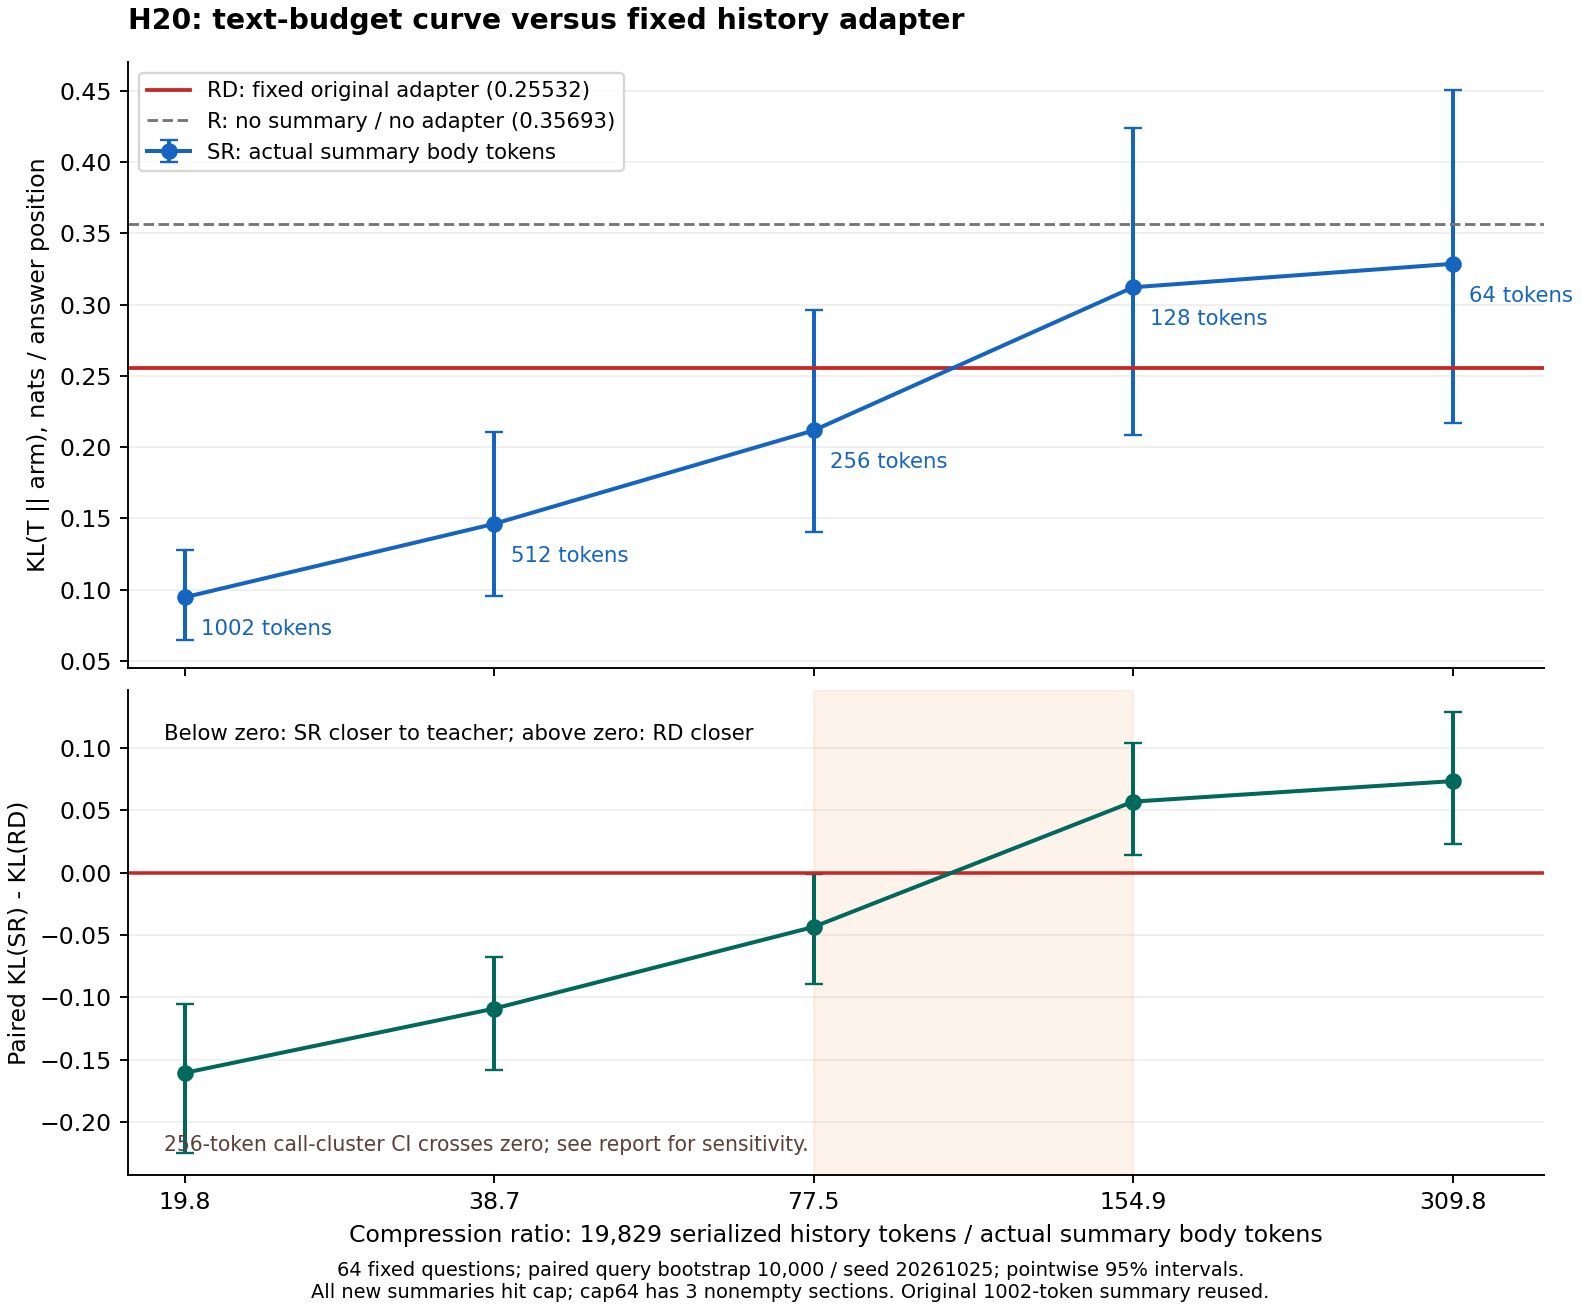
\includegraphics[width=0.86\textwidth]{figures/fig1-rstar}
\caption{$\KL(T\|\cdot)$ against the summary compression ratio $r$ on one 20k-token history. Upper panel:
summary carrier $\St{}$ (blue), fixed parameter carrier $\armRD{}$ (red), tail-only baseline (dashed). Lower
panel: the paired difference $\KL(T\|\St)-\KL(T\|\armRD)$; the shaded band marks the bracket of
\S\ref{sec:crossover}.}
\label{fig:rstar}
\end{figure*}

Two caveats follow from the construction. First, $r^\ast$ is a property of the quadruple (method, history,
summarization policy, probe set), not a universal constant: it depends on how compressible the particular history
is, on how the engine spends its budget, and---as \S\ref{sec:replication} shows---on which cells the write was
trained to answer, so changing only one of the four can move the crossing. Second, the direction of the
comparison at low $r$ is the expected one: at $r\approx 20$ the text carrier is unambiguously better.

\paragraph{Takeaway.} The sampled point estimates reverse order on all four histories: the text carrier is ahead
at wide budgets and the parameter carrier at narrow ones. The sign change lands anywhere between 10 and 256
tokens. H1's two endpoints exclude zero under both question- and cluster-level resampling; H20's two endpoints
exclude zero under question-level resampling, but its 256-token endpoint is sensitive to cluster resampling; the
short-history brackets for H2 and H3 remain uncertain.

\subsection{RQ3: The Price}\label{sec:cost}

A carrier that fits a distribution into weights perturbs everything those weights do, including questions that
never needed the history. Table~\ref{tab:replay} reports three quantities on the 32 unrelated questions, because
they answer three different objections: a distributional drift (how far behaviour on those questions moved), a
gold-NLL effect (whether the movement made the answers worse), and a greedy comparison (whether it changed any
answer at all).

The drift point estimate is larger than either text carrier's on the same questions (0.02587, against 0.01663 and
0.01597 for the two summaries), and the gold-NLL effect is positive with an interval excluding zero ($+0.0349$,
$[+0.0105,+0.0756]$). The paired intervals for the drift differences cross zero, so we report the ordering rather
than claim it. The greedy path is unchanged in every arm---31 of 32 correct, and never a correct-to-wrong
flip---so the drift we measure does not change answers: the gold likelihood moved while the measured greedy
outcomes did not. It also means the behavioural test has almost no headroom here, and we do not read its stability
as evidence of harmlessness.

\paragraph{Can the cost be trained away?} A cost that is only measured leaves the argument open, so we ran the
obvious remedy. Rehearsal interleaves the original write with updates on off-topic questions: every four history
updates are followed by one rehearsal update, so the adapter receives 64 history plus 16 rehearsal updates
instead of 64, with the rehearsal loss multiplied by $\lambda$. Both variants keep H20, the seed, the rank and the
layer set; $\lambda{=}0.5$ halves the loss weight, not the number of updates, and is not the same as halving the
optimiser step.

Both variants move the same way. At $\lambda{=}1$ the NLL effect becomes $-0.0016$, whose interval straddles
zero: the effect is no longer distinguishable from none, though the gate we had fixed---an upper bound at or
below zero---is still missed. The related side pays about a point (paired difference $-0.86$\,pp
$[-2.18,+0.69]$). Halving the loss weight is worse on both columns, so the trade does not improve by shrinking
the term. Neither variant meets both pre-registered conditions---a related-side non-inferiority bound of
$-2$\,pp on the paired lower interval, and an off-topic NLL upper interval at or below zero---and we do not
continue a $\lambda$ search on the sealed test.

\paragraph{What the three rows separate.} An effect that a weight update produced can also be reduced by another
weight update, so a rehearsal win says nothing by itself about where the cost comes from. What it does say is that
the effect is not inert: nine tenths of the drift and the detectable part of the NLL effect go away, at a price on
the related side. Within this setting---one history, one seed, two rehearsal weights---the measured side effect is
therefore sensitive to the training objective, and we report it that way; it does not identify an intrinsic lower
bound for parameter carriers.

\paragraph{Takeaway.} The write costs a drift on questions that never needed the history, larger than the two
summaries' point estimates, and rehearsal removes nine tenths of it for about a point of fidelity. The measured
side effect is sensitive to the training objective; neither pre-registered success condition was met.

\begin{table}[b]
\centering
\small
\setlength{\tabcolsep}{4pt}
\begin{tabular}{lrrr}
\toprule
Adapter & Related red. & Off-topic drift & Off-topic NLL \\
\midrule
$\armRD$, 64 updates & 28.47\% & 0.02587 & $+0.0349$ \\
$\armRD$ + replay $\lambda{=}1$ & 27.60\% & 0.00240 & $-0.0016$ \\
$\armRD$ + replay $\lambda{=}0.5$ & 27.11\% & 0.00316 & $+0.0059$ \\
\bottomrule
\end{tabular}
\caption{Cost of the write on H20, and the effect of rehearsal (64 history plus 16 rehearsal updates).}
\label{tab:replay}
\end{table}

\section{Discussion}

\subsection{Checks on Three Alternative Explanations}

\begin{enumerate}[leftmargin=1.2em]
\item \textbf{``The full-context teacher is degraded.''} On 32 unrelated questions at 50 gold positions,
$\KL(T\|\armR)=0.054753$, but the teacher's gold NLL difference relative to $\armR$ is $+0.009531$ with
interval [$-$0.008318, 0.026700], crossing zero. We therefore did not detect a difference in the teacher's
gold NLL on these questions: the interval is compatible with a small improvement as well as with a small
degradation. This
does not contradict the documented degradation of long-context performance
\cite{still2026}: our probe uses questions that do not require the far context, and it measures the teacher
against $\armR$ rather than a short-context-trained model against a long one.
\item \textbf{``The negative result on the summary channel is only a missing format template.''} Giving
all four arms the same eight-section heading template lowered every core cross-entropy but left the observed
ordering between arms essentially unchanged. The template
moves the floor rather than the ordering, so it does not account for the negative result on the summary channel.
\item \textbf{``Capacity is irrelevant.''} Reducing rank from 64 to 16 lowers the $\armR\to\armRD$ relative
reduction on H3 from 27.90\% to 20.03\%, a difference of $+7.87$\,pp with interval [5.55, 10.66] excluding
zero. Both figures come from the capacity scan on H3; its rank-64 reference is a frozen earlier fit, which is
why it reads 27.90\% here and 27.95\% in Table~\ref{tab:fit}. Capacity therefore has a measurable effect in
this configuration, but $4\times$ capacity buys about 8 points, the effect is undetectable on
$\St\to\Sd$, and with two ranks at one sampling condition we cannot rank it against the other unscanned
axes.
\end{enumerate}

\subsection{A Replication at Another Scale}\label{sec:replication}

A saturated write at this scale is expensive---2{,}304 updates, which is 64 passes over 36 training probes, plus a
full teacher pass per history---and it did not fit in the window of this version. We therefore ran the saturated
regime once, on
Qwen3.5-9B with its own history, question pool and summary method. The protocol is separate and
\textbf{its numbers must not be subtracted from, or pooled with, those of \S5}; it is a replication probe, not a
second experiment. What it shows is a shape, not a magnitude:

\begin{table}[t]
\centering
\small
\begin{tabular}{@{}l>{\raggedright\arraybackslash}p{5.3cm}@{}}
\toprule
Observation & 9B companion run \\
\midrule
Crossing & exists; interpolated at 540--650 summary tokens \\
Write budget & top-1 0.220$\to$0.497 and KL 0.7230$\to$0.7508, 4 to 64 passes \\
Probe coverage & a held-out single-field set stays at 0.31; covering it lifts it to 0.84 \\
Off-topic drift & not measured at saturation \\
\bottomrule
\end{tabular}
\caption{What the 9B companion adds.}
\label{tab:9b}
\end{table}

Three things carry over. The reversal exists there too, at a token count two to eight times our own, so what
replicates is the existence of a crossing rather than its position. The write budget matters below saturation, and
whether the two metrics move together depends on which pair of budgets is compared: on the 40-question evaluation,
four passes to 64 raise value-position top-1 from 0.220 to 0.497 while KL becomes slightly worse (0.7230 to
0.7508), whereas 16 to 64 improve both (0.288 to 0.497, KL 0.7661 to 0.7508). We therefore report the two metrics
side by side and never read one as the other. And at saturation the digit at a given position is
decodable from the adapter's own contribution, so ``fits a distribution'' is a matter of how much was written, not
a property of the
carrier (\S\ref{sec:limits}). What the run does not give us is a number for this model: the
27B saturated adapter does not exist, and until it does we cannot say whether the carrier closes its gap to a
summary (\S\ref{sec:cost}). Details---the decode probe, the axes that were not scanned, the exact protocol---are
in Appendix~\ref{app:9b}.

\paragraph{An intervention on what the probes ask about.} The companion probes a different axis from the one above.
With 56 training probes the adapter scored 0.3125 value-position top-1 on eight held-out single-field questions,
although those entities and their values had appeared in three-field training answers. Adding 24 single-field
probes in different wording raised the same score to 0.84375. That intervention changes the training distribution
\emph{and} the total number of updates (3{,}584 to 5{,}120), so it shows sensitivity to the entity--answer-format
coverage of the probe set; it does not isolate a factual coverage limit, nor a capacity limit. Wording sits on the other side of the comparison but in a separate run: in a 2{,}304-update
adapter, value-position top-1 was 0.969 on reworded three-field questions with the answer shape held fixed. These
tests show different sensitivities under the wording and answer-format changes we tried; they do not isolate a
general wording-versus-format distinction, and the three numbers come from three different checkpoints.

Two consequences we take seriously. First, the crossing moves with the probe set: the accuracy-based point
estimate is 6.76 on the 2{,}304-update adapter (the one that scored 0.969) and 4.20 on the 5{,}120-update
covered adapter (the one that scored 0.84375), a factor of 1.61 on that curve and indicator, not a capacity
ratio. This is a different pair from the 3{,}584-to-5{,}120 update intervention above---probe composition and
optimization exposure differ together---so it locates a sensitivity, not a probe-only effect. Second, our own
crossover in \S\ref{sec:crossover} is conditional on its own, sparse probe set; the direction and size of an
equivalent intervention at 27B are unmeasured.

\subsection{An Implication We Have Not Tested}

A session-local write leaves behind an auditable,
replayable record of what this history did to the model's distribution. Accumulated over many sessions,
such records would be the raw material a continual-learning procedure needs in order to cover behaviour
that today can only be obtained by training on long contexts. Our $\Delta$ itself does not accumulate---it
is session-local and discarded---so the collapse risk reported for multi-round internalization
\cite{collapse2026,shumailov2024} has no mechanism to act through here.

\subsection{Limitations}\label{sec:limits}

\begin{enumerate}[leftmargin=1.2em]
\item \textbf{Distribution fit is not a content claim.} $\Delta$ is fitted to the teacher's output distribution,
and every number in \S5 is a distributional distance. The companion shows sensitivity to training exposure and to
entity--answer-format coverage, but its intervention changes both probe composition and update count, so it does not
isolate their effects and we do not attribute the difference to coverage alone (\S\ref{sec:replication}). At 27B we
measured distributional fidelity, not independent table reconstruction or factual accuracy.
\item \textbf{No task-accuracy claim.} A smaller distributional distance does not imply task ability, and we do
not claim improved accuracy on any benchmark.
\item \textbf{The probe set is the weakest link, and we have no procedure for choosing one.} We draw 16 probes
uniformly, with no coverage criterion over the history's content, no sampling frame, and no sensitivity analysis
in their number or spread; a probe set that is too small, too clustered, or drawn from one part of the history
would look exactly like a limit of the carrier, and we cannot currently tell the two apart
(\S\ref{sec:threats}).
\item \textbf{A real cost on unrelated questions.} Writing a distribution into weights perturbs behaviour on
questions that do not need the history: on H20 the drift is 0.025874 against 0.016631/0.015966 for adding a
summary. Rehearsal reduces this drift by an order of magnitude at a small fidelity cost, but not for free
(\S\ref{sec:cost}).
\item \textbf{What the carrier answers depends on what the probes asked about.} On this history a summary whose body
is 1002 tokens is closer to the teacher than $\Delta$ alone (0.0946 vs 0.2553). In the companion, eight held-out
single-field questions scored 0.3125 once every answer shape had been trained, and 0.84375 after single-field
probes were added---an intervention that also changed the number of updates, so it bounds how much the reading
moves with the probe set without isolating which factor moved it (\S\ref{sec:replication}). How far the same holds
as histories grow in schema complexity is open.
\item \textbf{The write needs the block alive.} The teacher is $E{+}A{+}R{+}q$, so the write must happen before
$A$ is destroyed; an engine that has already discarded the block cannot be retrofitted without replaying it.
\item \textbf{One gradient write per session.} Sixty-four AdamW updates at the boundary are a per-session cost;
a hypernetwork over the history would amortize them~\cite{doctolora2026}, but that is a different mechanism and we did not build it.
\item \textbf{Session-local and non-accumulating.} $\Delta$ is discarded at session end, so nothing carries
across sessions; a procedure that did accumulate would face the collapse risk we cite
\cite{collapse2026,shumailov2024}.
\end{enumerate}

\subsection{Future Work}\label{sec:future}

Three things stand between these numbers and a method, in this order.

\paragraph{Choosing the probes.} This is the blocker, and the companion run says why: across the interventions we
tried, what a probe set asks about moved the reading more than anything else we varied, so the probe set is part of
the instrument rather than a neutral sample. Our 16 probes are drawn uniformly, cover few cells, and are validated
by no criterion, which makes a carrier that fails and a probe set that never asked about the right thing
indistinguishable (\S\ref{sec:limits}). The companion also shows the size of the prize: 24 extra one-field probes,
seven minutes of teacher and training time, raised a held-out set from 0.3125 to 0.84375
(\S\ref{sec:replication})---an intervention that also changed the update count, so the size of the prize is
established and its attribution is not. What is needed is a coverage model over the history's (entity, field)-style grid, a
stated sampling frame, and a sensitivity analysis in the number and the spread of probes---and, because coverage
changes the crossing, every $r^\ast$ in this literature should be reported with the probe set that produced it.

\paragraph{History diversity.} Our four histories are variants of one generator: same transaction grammar, same
kinds of questions, and four entities in H1--H3 against twelve in H20. The crossing location is measured on all
four and the rehearsal trade on H20 only, and we do not know whether either survives a history whose structure
differs---a codebase, a log stream, a long conversation with no typed fields. The relevant variation is
structural, not merely longer.

\paragraph{Model generality.} We have one base model at the target scale and one replication at a smaller scale
in a different protocol (\S\ref{sec:replication}). That is enough to show the shape is not an artifact of one
checkpoint, and not enough to say where the crossing sits for another model. The next run should be the same
five-arm protocol on a second model at the same scale, not another arm on this one.

\section{Related Work}\label{sec:related}

Stated up front: every line of work below is successful on its own problem, and this section
\textbf{does not rank them}. Table~\ref{tab:matrix} applies the four criteria of \S\ref{sec:criteria} to
representative systems from four families; the judgment behind each row is argued in the subsection below,
not in the table.

\begin{table*}[t]
\centering
\footnotesize
\setlength{\tabcolsep}{4pt}
\begin{tabularx}{\textwidth}{@{}>{\raggedright\arraybackslash}p{3.6cm}>{\raggedright\arraybackslash}p{1.3cm}>{\raggedright\arraybackslash}X>{\raggedright\arraybackslash}X>{\raggedright\arraybackslash}p{1.9cm}>{\raggedright\arraybackslash}p{1.6cm}@{}}
\toprule
Work & A write point & B carrier $=$ params & C supervision & A$'$ lifecycle (given A) & Reading \\
\midrule
Current engine (text compaction) & \checkmark & $\times$ summary $+$ window & --- & --- & A only \\
Still / RestoreKV & \checkmark & $\times$ edits KV & \checkmark\ KL & $\times$ prefix-bound & no B \\
Cartridges / SemPIC~\cite{sempic2026} / xKV~\cite{xkv2025} & $\times$ & $\times$ compact KV & \checkmark\ distillation & n/a & no A, no B \\
LOHA/ACD & \checkmark & $\times$ soft tokens & \checkmark\ per-token KL & $\times$ dies with context & no B \\
REMORY & \checkmark & $\times$ soft tokens & \checkmark\ reverse KL & $\times$ $\Delta{\neq}0$ & no B \\
CCM~\cite{ccm} & \checkmark & $\times$ retained memory in prompt & \checkmark\ privileged full-history distillation & --- & no B \\
LCLM~\cite{lclm2026} & $\times$ & $\times$ latent tokens & $\times$ token CE & n/a & spatial \\
RLM~\cite{rlm2025} / StateLM~\cite{statelm2026} / DocAtlas~\cite{docatlas2026} & $\times$ & $\times$ read back into context & --- & --- & spatial \\
RPMem / Doc-to-Atom / ASCENT~\cite{ascent2026} & $\times$ & \checkmark & \checkmark\ contextual KL & --- & no A \\
DPPM & $\times$ & \checkmark & $\times$ CE on answers & --- & write point \\
Doc-to-LoRA & $\times$ & \checkmark & \checkmark\ context distillation & --- & write point \\
Language Models Need Sleep~\cite{sleep2026} & $\times$ & \checkmark\ merged into base & \checkmark\ on-policy distillation & $\times$ permanent & no A \\
Sleeping LLM (Zenodo)~\cite{perfact} & $\times$ & \checkmark\ per-fact LoRA & $\times$ per-fact edits, not a distribution & $\times$ permanent & B only \\
TMEM & \checkmark & \checkmark\ LoRA & $\times$ JSON-QA $\to$ SFT & \checkmark\ per-episode & no C \\
\midrule
\textbf{This work} & \checkmark\ \textbf{compaction}\newline \textbf{boundary} & \checkmark\ \textbf{parameters, no window} & \checkmark\ \textbf{direct full-vocab fit} & \checkmark\ \textbf{$\Delta{=}0$, discard} & --- \\
\bottomrule
\end{tabularx}
\caption{The four criteria of \S\ref{sec:criteria} applied to representative systems from four families.
$\checkmark/\times$ mark satisfaction only, with no quality ranking; ``---'' means the work does not state it;
rows are not exhaustive.}
\label{tab:matrix}
\end{table*}

\subsection{Compiling Context into Parameters: the Bounded-Document Regime}

Doc-to-LoRA \cite{doctolora2026} uses a hypernetwork to compile a context into a LoRA adapter in a single
forward pass, amortizing the gradient step away; RPMem \cite{rpmem2026} substitutes a stronger
hypernetwork backbone (session $\to$ latent code $\to$ LoRA); DPPM \cite{dppm2026} runs an
evidence-plus-delta dual path; Doc-to-Atom \cite{doctoatom2026} uses atom-level micro-LoRAs with routing;
Memory Depth \cite{memdepth2026} gates LoRA writes by surprise and valence. Their write points are at the
end of a session, a task, a document, or a number of rounds; ours is at the moment history is destroyed.
These are different trigger conditions, so the comparison below is not a contest on the same question.

This family already evaluates inference \emph{without} the original context: Doc-to-LoRA's retrieval evaluation
gives the target model only the query, and the adapter is what carries the document \cite{doctolora2026}. So
``the text is gone and only the parameters remain'' is not what separates our work from theirs. What differs is the trigger and the measurement: their write point is a task, document or session
boundary, ours is the moment the engine destroys the block; and we compare carriers against a real
summary-generation policy across swept token budgets.

Our write point is triggered by imminent death of the context: in the \armRD{} arm, $A$ has already been
removed and $\Delta$ is its \emph{only} carrier. The question becomes ``can parameters replace text that
no longer exists?'' Hence the control arm, the cost structure, and the failure modes all differ.

A reported cost of this family: Doc-to-LoRA-style methods collapse to 46.4\% when the context conflicts
with pretrained priors \cite{overridegap2026}. We have not tested such conflicts and record this as
uncovered, rather than as a risk already avoided.

\subsection{TMEM at the Episode Boundary: the Nearest Neighbor}

TMEM \cite{tmem2026}---\emph{Scaling Self-Evolving Agents via Parametric Memory}---is the closest neighbor: episode-boundary trigger, online LoRA, true identity at
$B{=}0$, context cleared after the write. The difference is one thing: \textbf{its supervision first
passes through a JSON-QA extraction}. Consequently $\Delta$ learns what the extractor can ask
about---facts never asked, dispositions that cannot be phrased, cross-event consistency do not enter the
supervision channel. That step also buys something: text-form supervision is inspectable, attributable,
and refusable. The accurate phrasing is therefore not that it ``adds a step'', but that the two schemes
\emph{differ in their supervision channel}: one is mediated by an extractor, the other is a direct distribution
over answer positions. Whether the direct channel in fact carries more usable information is a hypothesis we have
not measured---our own supervision is itself bounded by the probe set (\S\ref{sec:limits}), so ``more bandwidth''
would need its own experiment.

\subsection{Keeping History on the Token Side}

Another line keeps compressed history on the token/KV side: Cartridges compiles context into a compact KV
offline \cite{cartridges2025}, and naive mixing of independently trained cartridges collapses to random
\cite{cartridges_scale2026}; REMORY uses bounded soft memory tokens \cite{remory2026}; LOHA/ACD compresses
old observations into soft tokens (SWE-bench 12.1/21.8 versus 14.5/27.5 uncompressed) \cite{loha2026}; its
anchored distillation is a distribution match, as ours is, but the two write different things: ACD trains a
reader for a carrier that stays in the sequence, whereas here the distillation writes the carrier itself and
the history leaves the sequence. REMORY makes the same point more sharply: it distils at the compaction
boundary itself and still writes soft tokens. Neither is a substitute for us on cost: both keep the compressed
history in the sequence, so they consume window positions and pay attention work proportional to the number of
tokens they inject (\S1.2).
Still compresses KV recursively with per-layer Perceivers \cite{still2026}; RestoreKV restores evicted KV
with a LoRA \cite{restorekv2026}. These methods are effective, and are the natural choice in the regime
where windows are wide enough. Their cost item is tokens or KV, so in the regime where the window itself
is the constraint the constant is what shrinks---KV compression buys headroom, not independence from the number
of positions still carried (\S1.2).

\subsection{Parameter versus KV: What Prior Comparisons Say}

In fairness, parameters do not win at \emph{retrieval}: EVAF \cite{evaf2026} reports factual retrieval of
0.956--0.973 versus 0.812--0.904 for parameter internalization, and \cite{doclive2026} reports KV about
10 points above parameters at matched budget, with parameters the only arm showing catastrophic
forgetting. We claim only that the \emph{cost shape}
differs, so in the regime where the text budget has to stay small the parameter carrier has budget left, at the
fidelity we measured. This is also
why we must report drift on unrelated questions---a cost identified in \cite{doclive2026}---and we list it
separately rather than omitting it.

\section{Threats to Validity}\label{sec:threats}

\paragraph{Construct.} The primary metric is distributional distance, not task accuracy: on the 32
unrelated questions the greedy accuracy is 31/32, leaving no headroom, and related questions have no gold
independent of the teacher, so \textbf{no task-level effect is established}. The metric also does not say which
part of an answer a difference is carried by: the full-vocabulary KL is taken over surface tokens and is not
decomposed into the typed values of the histories (\S\ref{sec:histories}) and the surface form that expresses
them. A distributional distance can also look satisfactory while behaviour does not: in the companion run of
\S\ref{sec:replication}, going from four to 64 passes doubles value-position top-1 (0.220 $\to$ 0.497) while KL
becomes slightly worse (0.7230 $\to$ 0.7508). The two metrics answer different questions, so we report them side
by side and never read one as the other.
\paragraph{Internal.} (i) The training set is 16 probes, drawn uniformly by us, with \textbf{no coverage
criterion and no probe-quality measure}; their sampling variance is not measured, so every conclusion about
capacity and step count is conditional on one draw of one size, and we cannot separate a carrier limit from a
probe limit (\S\ref{sec:limits}). The companion gives the size of that hole: covering the same cells with
question-phrased probes raises a held-out cell from 0.31 to 0.84, so the 16 probes here are not a neutral choice.
(ii) Only four
generation clusters; no multiplicity correction; intervals are conditional on a fixed question pool. (iii)
Unscanned axes: layer placement, teacher target length, probe count (scanned: rank 16/64, updates 0/16/64/256,
i.e.\ at most 16 passes per probe; the companion run (\S\ref{sec:replication}) scans to 64 passes at 9B and finds the budget
decisive). Table~\ref{tab:knobs} lays out the whole space and what of it we moved.
(iv) The three invariants of \S\ref{sec:notation} are enforced by construction and verified by hash, but we did
not run a deliberately violated arm, so we cannot bound how much of a paired difference a violation would
absorb.
\paragraph{External.} Four constructed histories, a single 27B base model, a single GPU; the entropy and noise
structure of real sessions are not covered.
\paragraph{Measured, and not measured.} Drift was measured on one history and one seed. The write side was not
instrumented: we report parameters, bytes and update counts (\S\ref{sec:costmodel}), not wall clock, peak memory
or first-token latency. And the cost was measured at the budget we fit, so whether it grows as the adapter
saturates is open (Appendix~\ref{app:9b} records the same gap)---which is where a rehearsal trade would break
first.
\paragraph{Scope of the runs.} The artifact is small; studying it is not. One saturated write is
2{,}304 updates (64 passes over 36 probes) plus a teacher pass over the full history, and every arm of every sweep
needs its own cold pass; the engineering around state handling, prefix caching and byte-exact verification cost
more than the GPU hours did. We therefore did not finish the study: the 27B ladder stops at 16 passes per probe,
the saturated regime is reported from a 9B companion rather than from this model
(\S\ref{sec:replication}), and a second seed, a matched-budget cost comparison and a wider history set were not
run. What is missing is missing because of cost, not because the hypothesis was dropped, and we prefer to say so
than to fill the space with runs that cannot be compared.

\section{Conclusion}

We asked whether the carrier of history across a compaction boundary can be parameters rather
than text, and measured the answer instead of arguing it. At the boundary we write the full-context teacher's
output distribution into a session-local, unmerged low-rank $\Delta$ that is bitwise identity when cleared. On a
single 27B model over four constructed histories the write reduces the divergence from the teacher by
25.1/28.0/28.5\% over the tail-only baseline, by 7.7\% on a fourth history whose interval crosses zero, and by
17.8\% on top of a summary on one history. On a 20k-token history the text carrier stays closer until the
summary is compressed to 128--256 tokens, where the comparison reverses. On the three shorter histories the sampled
point estimates reverse order again, at budgets between 10 and 200 tokens, but only one of the three is bracketed by
two endpoints whose intervals both exclude zero, so we report no transferable crossing location. On questions
that do not need the
history, $\Delta$ costs 0.026 nats/position against 0.017 for adding a summary. What this establishes is that
the state can live in parameters and what that costs; at the write budget used here a summary of comparable
length is still closer to the teacher than $\Delta$ alone, so the claim is about where the state lives, not
about replacing text.

\section*{Data Availability}

Each table has a manifest listing the input files it was computed from, the raw tensors, and the
SHA-256 digests and base-model commit hash of both; the manifests and statistics scripts are available from the
authors on request. The base model is pinned at
\texttt{1d4bf0f2ff6012fd82039f2fa52739d0dd7c60c0}.

\appendix
\section{A Companion Study at 9B}\label{app:9b}

A second study, run on Qwen3.5-9B on a single 22~GiB GPU, repeats the measurement on a 36-entity service table
with its own question pool. The protocol is separate, so \textbf{its numbers must not be compared with those in
\S\ref{sec:results}}. It exists because the saturated regime does not fit at 27B: 2{,}304 updates over 36 probes
plus a teacher pass over the full history is a different order of cost from the 64-update write we study
here, and a 9B run was the only way to see that regime inside this version's budget. We report it because it
bears on three claims made above; the summary in the main text is \S\ref{sec:replication}.

\paragraph{Crossing.} A log-$r$ interpolation between the same two sampled endpoints places the crossing at
$r^\ast\approx5.5$ by KL and $\approx6.8$ by value-position top-1 (5.85 on rephrased questions), i.e.\ 540--650
summary tokens. The sampled bracket is wider: it spans the 512- and 1024-token budgets, two to eight times the
128--256 tokens of \S\ref{sec:crossover}. The \emph{form} of the result reproduces; the token count does not
transfer across models.

\paragraph{Write budget.} Holding everything else fixed and varying the number of passes per supervised entity,
the trained-wordings value-position top-1 of the fitted adapter moves from 0.32 at four passes to 1.000 at 64, with the
rephrased-question top-1 moving from 0.20 to 0.59 and then saturating (a further $2\times$ of steps: 0.59). Over
the same range KL moves the wrong way: from four passes to 64, top-1 on the 40-question set rises 0.220 $\to$
0.497 while $\KL(T\|\cdot)$ rises (gets worse) 0.7230 $\to$ 0.7508. We report the two side by side and do not
read either as the other; we also do not conclude that KL is broken, since the two answer different questions (a
full distribution versus the top-1 token), and the cause of the divergence is not decomposed here.

\paragraph{Coverage.} The two runs behind \S\ref{sec:replication} differ in what the probes asked about, and also in
the number of updates, which is why neither isolates coverage alone. The first trains every answer shape---36
three-field, 12 two-field and 8 one-field probes on a rotated field, 3{,}584 updates---and holds out eight
one-field questions on other entities. The second keeps those shapes and adds 24 one-field probes, in our own
wording, on the entities whose single-field questions had not been asked (80 probes, 5{,}120 updates). Adding
those 24 probes cost 173\,s of teacher targets and 224\,s of training. Drift and the rank and layer axes were scanned at the low
budget only, and no 27B run at the larger budget exists, so whether the carrier of \S\ref{sec:results} closes its
gap to a summary when trained further is open.

\paragraph{Decode.} At the position where a digit is emitted, a linear classifier decoded the next digit from the
adapter's contribution to the MLP output at 0.928 accuracy, on 250 teacher-forced digit positions from 36 probes,
against 0.472 from base-MLP features collected in the same forward pass and a 0.192 majority-class baseline. This
establishes conditional decodability at those positions; it is not reconstruction of the table from the adapter
weights alone.

% Bibliography is generated by BibTeX from references.bib.
% Style: ACM-Reference-Format (ships with the acmart class; the
% expected style for acm conference proceedings).
% ACM requires this style; it numbers entries alphabetically by author, so [n] is not the order
% of appearance. Kept as-is: format compliance wins over reading order.
\bibliographystyle{ACM-Reference-Format}
\bibliography{references}

\end{document}
